\textbf{12.1.1.} 试论证:平行板电容器必定有边缘效应, 换句话说, 在两极板间电场是均匀的, 而到外边电场突然变为零[像图 12.1.1(1)那样], 是不可能的.

图12.1.1(1)

图12.1.1(2)

【论证】作一长方形环路 $L$ ，使其长为 $l$ 的两对边平行于电场强度 $\pmb{E}$ ，且一边在电场内，另一边在电场外，如图12.1.1(2)所示，则根据题目所说条件， $\pmb{E}$ 沿 $L$ 的环量为

$$
\oint_ {L} \boldsymbol {E} \cdot \mathrm{d} \boldsymbol {l} = E l\tag{1}
$$

对于静电场来说，对任何环路 L 都有

$$
\oint_ {L} \boldsymbol {E} \cdot \mathrm{d} \boldsymbol {l} = 0\tag{2}
$$

这是静电场的基本性质。现在式(1)不满足式(2)，说明式(1)不对。但式(1)在计算上并无问题，可见问题出在条件上，即题目所说的条件（在两极板间电场是均匀的，而到外边电场突然变为零）是不对的。也就是说，像图12.1.1(1)那样的静电场是不存在的。
\begin{center}
    
\includegraphics[width=0.5\linewidth]{figures/fig_12_1_1_1.jpg}
\end{center}
\begin{center}
    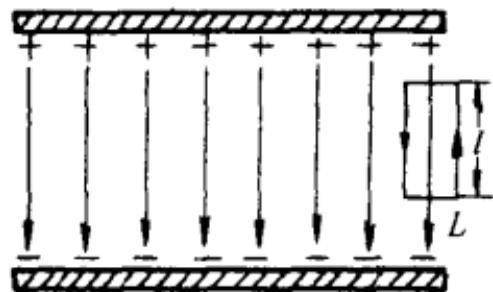
\includegraphics[width=0.5\linewidth]{figures/fig_12_1_1_2.jpg}
\end{center}

\vfill

\textbf{12.1.2.} 试论证:磁铁必定有边缘效应, 换句话说, 在两极间磁场是均匀的, 而到外边磁场突然变为零[像图 12.1.2(1)那样], 是不可能的.

【论证】作一长方形环路 $L$ ，使其长为 $l$ 的两对边平行于磁场强度 $\pmb{H}$ ，且一边在磁场内，另一边在磁场外，如图12.1.2(2)所示，则根据题目所说条件， $\pmb{H}$ 沿 $L$ 的环量为

$$
\oint_ {L} \boldsymbol {H} \cdot \mathrm{d} \boldsymbol {l} = H l\tag{1}
$$

对于静磁场来说，对任何环路 L 都有

$$
\oint_ {L} \boldsymbol {H} \cdot \mathrm{d} \boldsymbol {l} = I\tag{2}
$$

式中 $I$ 是环路 $L$ 所套住的自由电流的代数和. 式(2)就是安培环路定理, 是磁场的基本规律. 将这定理用于图12.1.2(2)中的环路 $L$ , 便得

图12.1.2(1)

图12.1.2(2)

$$
\oint_ {L} \boldsymbol {H} \cdot \mathrm{d} \boldsymbol {l} = 0\tag{3}
$$

式(1)不满足式(3)，说明式(1)不对.但式(1)在计算上并无问题，可见问题出在条件上，即题目所说的条件(在两极间磁场是均匀的，而到外边磁场突然变为零)是不对的.也就是说，像图12.1.2(1)那样的静磁场是不存在的.
\begin{center}
    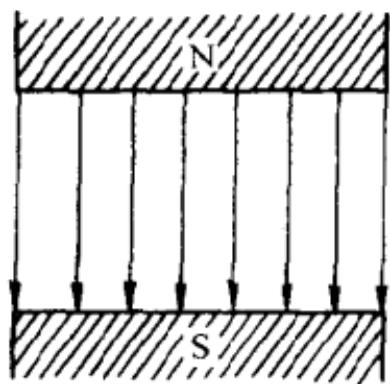
\includegraphics[width=0.5\linewidth]{figures/fig_12_1_2_1.jpg}
\end{center}
\begin{center}
    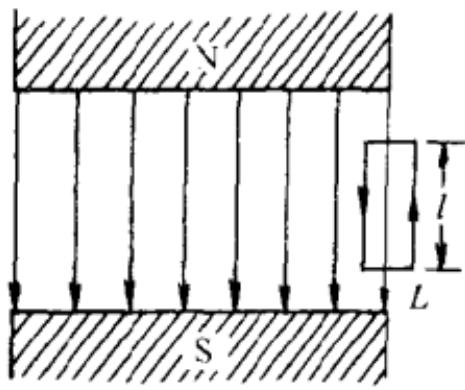
\includegraphics[width=0.5\linewidth]{figures/fig_12_1_2_2.jpg}
\end{center}

\vfill

\newpage

\textbf{12.1.3.} 试证明: 略去边缘效应时, 平行板电容器中的位移电流为 $I_{D} = \varepsilon S \frac{\mathrm{d} E}{\mathrm{d} t}$ , 式中 $\varepsilon$ 是两极板间介质的电容率, $S$ 是极板的面积, $E$ 是极板间电场强度的大小.

\vfill

\textbf{12.1.4.} 一空气平行板电容器的两极板都是半径为 $5.0\mathrm{cm}$ 的圆形导体片，在充电时，其中电场强度的变化率为 $\frac{\mathrm{d}E}{\mathrm{d}t} = 1.0\times 10^{12}\mathrm{V / (m\cdot s)}$ .略去边缘效应，试求：(1）两极板间的位移电流 $I_{D}$ ；(2）两极板边缘处磁感强度 $\pmb{B}$ 的值.

\vfill

\newpage

\textbf{12.1.5.} 一平行板电容器两极板间充满弱导电的均匀介质，当它充电后，断开电源，电荷便经过介质渐渐漏掉。略去边缘效应，试求漏电时两极板间的磁场。

\vfill

\textbf{12.1.6.} 当导线中载有交流电时，试证明：其中传导电流密度 $j$ 与位移电流密度 $\frac{\partial D}{\partial t}$ 的大小之比为 $\sigma / \omega \varepsilon_0$ ，式中 $\sigma$ 是导线的电导率， $\omega = 2\pi \nu$ ， $\nu$ 是交流电的频率，金属导体的 $\varepsilon_r$ 可当作1。已知铜的电导率为 $\sigma = 5.9 \times 10^7 \mathrm{~S} / \mathrm{m}$ ，试分别计算铜导线中载有频率为(1)50Hz和(2) $3.0 \times 10^{11} \mathrm{~Hz}$ 的交流电时，传导电流密度与位移电流密度的大小之比。

\vfill

\newpage

\textbf{12.1.7.} 一无穷长直螺线管，横截面的半径为 $R$ ，由表面绝缘的细导线密绕而成，单位长度的匝数为 $n$ .当导线中载有交流电流 $I = I_0\sin \omega t$ 时，试求管内外的位移电流密度的大小.

\vfill

\textbf{12.1.8.} 一圆柱形无穷长直导线，半径为 $a$ ，载有稳恒直流 $I$ ， $I$ 均匀地分布在横截面上.试求这导线内外磁场强度 $\pmb{H}$ 的旋度 $\nabla \times \pmb{H}$

\vfill

\newpage

\textbf{12.1.9.} 在一圆柱形空间内，有均匀的、但是随时间 $t$ 变化的磁场，其磁感强度为 $\pmb{B} = B(t)\pmb{k}$ ， $\pmb{k}$ 是沿圆柱轴线方向上的单位矢量。取笛卡儿坐标系如图12.1.9(1)所示，试证明：在此柱体内离轴线为 $r = \sqrt{x^2 + y^2}$ 处，电场强度为 $\mathbf{E} = \frac{1}{2} (y\mathbf{i} - x\mathbf{j})\frac{\mathrm{d}B}{\mathrm{d}t}$ .

\vfill

\textbf{12.1.10.} 在半径为 R 的圆筒内，有方向与轴线平行的均匀磁场，这磁场的磁感强度 B 以 100Gs/s 的速率减小。筒内有一电子，到轴线的距离为 r = 5.0cm，如图 12.1.10 所示。已知电子的质量为 $m = 9.1 \times 10^{-31}$ 千克，电荷量为 $e = -1.6 \times 10^{-19}C$ 。试求这电子的加速度。若这电子处在圆筒的轴线上，它的加速度是多少？
\begin{center}
    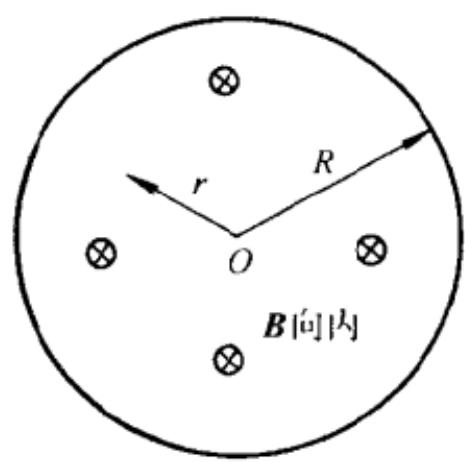
\includegraphics[width=0.5\linewidth]{figures/fig_12_1_10.jpg}
\end{center}

\vfill

\newpage

\textbf{12.1.11.} 一很长的直圆筒，半径为 $R$ ，表面上带有一层均匀电荷，电荷量的面密度为 $\sigma$ .在外力矩的作用下，从 $t = 0$ 时刻开始，以匀角加速度 $\alpha$ 绕它的几何轴转动，如图12.1.11所示.(1)试求筒内的磁感强度 $\pmb{B}$ ;(2)试求筒内接近内表面处的电场强度 $\pmb{E}$ 和坡印亭矢量 $\pmb{S}$ ;(3)试证明：进入这圆筒长为 $l$ 一段的 $\pmb{S}$ 的通量等于 $\frac{\mathrm{d}}{\mathrm{d}t}\left(\frac{\pi R^2l}{2\mu_0} B^2\right)$

\vfill

\textbf{12.1.12.} 试证明:麦克斯韦方程组的解满足叠加原理,即若 $E_{i}$ 、 $D_{i}$ 、 $H_{i}$ 、 $B_{i}$ 满足场源为 $\rho_{i}$ 和 $j_{i}$ 的麦克斯韦方程组,则 $\sum_{i=1}^{n} E_{i}$ 、 $\sum_{i=1}^{n} D_{i}$ 、 $\sum_{i=1}^{n} H_{i}$ 、 $\sum_{i=1}^{n} B_{i}$ 便满足场源为 $\sum_{i=1}^{n} \rho_{i}$ 和 $\sum_{i=1}^{n} j_{i}$ 的麦克斯韦方程组.

\vfill

\newpage

\textbf{12.1.13.} (1) 在空间取一任意封闭曲面 $S$ ，它所包住的体积为 $V$ ，用一任意曲面 $S'$ 把 $V$ 分隔为两部分，因此 $S$ 被分成 $S_1$ 和 $S_2$ 两部分，而 $S_1 + S'$ 和 $S_2 + S'$ 便都是封闭曲面，如图 12.1.13(1) 所示。试证明：若电场的高斯定理

(1)

图12.1.13

$$
\oiint_ {S} \boldsymbol {D} \cdot \mathrm{d} \boldsymbol {S} = Q
$$

和磁场的高斯定理

$$
\oiint_ {S} \boldsymbol {B} \cdot \mathrm{d} \boldsymbol {S} = 0
$$

对于 $S_{1} + S'$ 和 $S_{2} + S'$ 都成立，则它们对于 S 也必定成立.

(2) 在空间取一条任意闭合曲线 $L$ ，过其上任意两点作任一曲线 $L'$ ， $L'$ 将 $L$ 分成 $L_1$ 和 $L_2$ 两段，而 $L_1 + L'$ 和 $L_2 + L'$ 便都是闭合曲线，如图12.1.13(2)所示。试证明：若法拉第电磁感应定律

$$
\oint_ {L} \boldsymbol {E} \cdot \mathrm{d} \boldsymbol {l} = - \frac {\mathrm{d} \Phi}{\mathrm{d} t}
$$

和安培环路定理

$$
\oint_ {L} \boldsymbol {H} \cdot \mathrm{d} \boldsymbol {l} = I + \frac {\mathrm{d} \Phi_ {D}}{\mathrm{d} t}
$$

对于 $L_{1} + L^{\prime}$ 和 $L_{2} + L^{\prime}$ 都成立，则它们对于 $L$ 也必定成立.
\begin{center}
    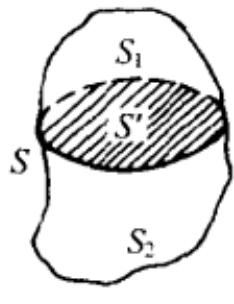
\includegraphics[width=0.5\linewidth]{figures/fig_12_1_13_1.jpg}
\end{center}
\begin{center}
    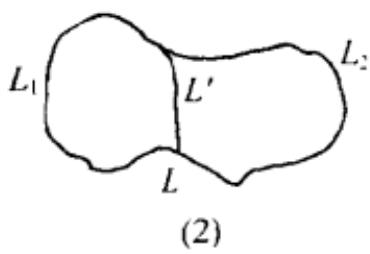
\includegraphics[width=0.5\linewidth]{figures/fig_12_1_13_2.jpg}
\end{center}

\vfill

\textbf{12.1.14.} 试由麦克斯韦方程组证明: 在介电常数 $\varepsilon_r$ 和相对磁导率 $\mu_r$ 都是常数的均匀介质中, 当自由电荷量密度 $\rho$ 和自由电流密度 $j$ 均为零 (即纯粹电磁场)时, $E$ 和 $H$ 都满足波动方程 $\nabla^2 F - \frac{1}{v^2} \frac{\partial^2 F}{\partial t^2} = 0$ , 式中 $v = \frac{1}{\sqrt{\varepsilon_r \mu_r \varepsilon_0 \mu_0}}$ 是电磁波在该介质中的速度.

\vfill

\newpage

\textbf{12.1.15.} 试由麦克斯韦方程组导出电荷守恒定律：

$$
\nabla \cdot \boldsymbol {j} + \frac {\partial \rho}{\partial t} = 0.
$$

\vfill

\textbf{12.1.16.} 电磁场的边值关系为:在两个介质交界面的两边上,(1)电场强度E的切向分量相等;(2)磁感强度B的法向分量相等;(3)当交界面上无自由面电荷时,电位移D的法向分量相等;(4)当交界面上无自由面电流时,磁场强度H的切向分量相等.试由麦克斯韦方程推出上述关系.

\vfill

\newpage

\textbf{12.1.17.} 两介质的电容率和磁导率分别为 $\varepsilon_{1},\mu_{1}$ 和 $\varepsilon_{2},\mu_{2}$ ，在它们的交界面上既无自由电荷，亦无自由电流；在交界面两边，电场强度与交界面法线的夹角分别为 $\theta_{1}$ 和 $\theta_{2}$ ，磁场强度与交界面法线的夹角分别为 $\varphi_{1}$ 和 $\varphi_{2}$ ，如图12.1.17所示。试证明： $\varepsilon_{1} \cot \theta_{1} = \varepsilon_{2} \cot \theta_{2}, \mu_{1} \cot \varphi_{1} = \mu_{2} \cot \varphi_{2}$ 。

图12.1.17
\begin{center}
    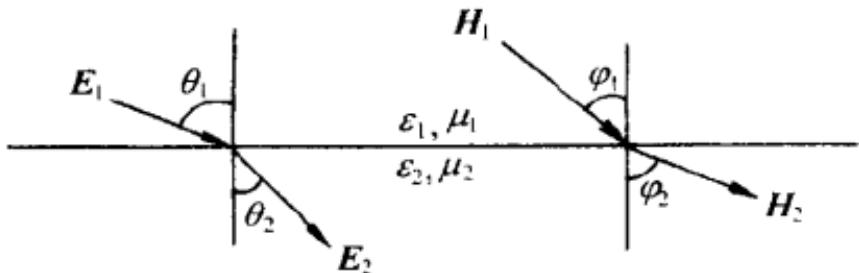
\includegraphics[width=0.5\linewidth]{figures/fig_12_1_17.jpg}
\end{center}

\vfill

\textbf{12.1.18.} 试论证: 理想导体(即电阻率 $\rho = 0$ 的导体) 表面外附近的电场强度总是与表面垂直.

【论证】由 $j = \sigma E = \frac{1}{\rho} E$ 知，理想导体内的电场强度为

$$
\boldsymbol {E} = \rho \boldsymbol {j} = 0
$$

根据电场强度的边值关系[参见前面12.1.16题的式(6)]，在交界面两边，电场强度 $\pmb{E}$ 的切向分量相等. 今理想导体内 $E = 0$ ，故 $\pmb{E}$ 的切向分量亦为零，于是理想导体表面外附近电场强度的切向分量亦应为零. 所以理想导体表面外附近的电场强度总是与表面垂直.

\vfill

\newpage

\textbf{12.1.19.} 金属的电导率为 $\sigma$ ，介电常数为 $1$ （即 $\varepsilon_{\mathrm{r}} = 1$ ）。设在 $t = 0$ 时刻，金属中某点的自由电荷量密度为 $\rho_0$ ，试求 $t$ 时刻该点的自由电荷量密度 $\rho(t)$ 。已知 $\varepsilon_0 = 8.854 \times 10^{-12} \mathrm{~F/m}$ ，铜的电阻率为 $1.7 \times 10^{-8} \Omega \cdot \mathrm{m}$ ，试计算铜内自由电荷量密度从 $\rho_0$ 减小到 $\frac{\rho_0}{\mathrm{e}} = \rho_0 / 2.71828$ 所需的时间 $\tau$ （ $\tau$ 通常叫做弛豫时间）。

\vfill

\textbf{12.1.20.} 将麦克斯韦方程组写成积分形式，然后用于稳定的直流电路，从而导出基尔霍夫电路方程组：(1) 每个分支点 $\sum_{i} I_{i} = 0$ ; (2) 每个回路 $\sum_{i} U_{i} = \sum_{i} E_{i}$ .

\vfill

\newpage

\textbf{12.1.21.} 在我们所使用的国际单位制里， $\nabla \cdot D = \rho$ ，库仑定律为 $F = \frac{1}{4\pi\varepsilon_0}$ $\frac{q_1q_2}{r^3} r$ ；在高斯单位制里， $\nabla \cdot D = 4\pi\rho$ ，试问在高斯单位制里，库仑定律的形式如何？

【解答】在高斯单位制里， $\nabla \cdot D = 4\pi \rho$ ，对于一个电荷量为 $q$ 的点电荷，利用高斯公式得

$$
\begin{array}{r l} \iint_ {S} \boldsymbol {D} \cdot \mathrm{d} \boldsymbol {S} & = 4 \pi r ^ {2} D = \iiint_ {V} \nabla \cdot \boldsymbol {D} \mathrm{d} V = 4 \pi \iiint \rho \mathrm{d} V \\ & = 4 \pi q \end{array}
$$

故得

$$
\boldsymbol {D} = \frac {q}{r ^ {3}} \boldsymbol {r}
$$

在高斯单位制里，在真空中 D = E，故得

$$
\boldsymbol {E} = \frac {q}{r ^ {3}} \boldsymbol {r}
$$

于是得高斯单位制里库仑定律的形式为

$$
\boldsymbol {F} = \frac {q _ {1} q _ {2}}{r ^ {3}} \boldsymbol {r}
$$

## § 12.2 电磁波

\vfill

\textbf{12.2.1.} 在空气中有一个单色平面电磁波, 它的频率为 $1.0 \times 10^{8}$ Hz, 位移电流密度的方均根值为 $1.0 \times 10^{-5}$ A/m². 试求这电磁波的电场强度和磁场强度的振幅 $E_{0}$ 和 $H_{0}$ .

\vfill

\newpage

\textbf{12.2.2.} 已知真空中一平面电磁波的电场强度为 $E = E_0\mathrm{e}^{\mathrm{i}(k\cdot r - \omega t)}$ ，式中 $E_0$ 是常矢量， $\omega$ 是圆频率， $\pmb{k}$ 是传播矢量， $\pmb{r}$ 是位置矢量， $i = \sqrt{-1}$ ，e是自然对数的底．试由麦克斯韦方程求这电磁波的磁场强度 $\pmb{H}$

\vfill

\textbf{12.2.3.} 在一平面电磁波里，同一点电场强度和磁场强度的振幅有如下关系： $\sqrt{\varepsilon} E_0 = \sqrt{\mu} H_0$ 。（1）试由此证明：(i)在平面电磁波里，电场能量的密度与磁场能量的密度相等；(ii)在真空中，电磁波磁感强度的振幅为 $B_{0} = E_{0} / c$ ， $c$ 为真空中光速。（2）在离一无线电台几公里处，该电台发出的电磁波在小范围内近似于平面波，它的 $E_0 = 0.10\mathrm{V / m}$ ，试求该处这电磁波的 $B_{0}$ 的值。

\vfill

\newpage

\textbf{12.2.4.} 真空中，一带电粒子在平面电磁波里运动，试证明：电磁波的电场作用在它上面的力大于电磁波的磁场作用在它上面的力.

\vfill

\textbf{12.2.5.} 一平面线圈的面积为 $0.50 ~m^{2}$ ，共有 5 匝，放在频率为 $2.0 ~MHz$ 的电磁波里，它的方位是使电磁波在它里面产生的感应电动势为最大，设这时感应电动势的有效值为 $10 ~mV$ ，试求该电磁波的磁场强度 H 的振幅。

\vfill

\newpage

\textbf{12.2.6.} 当太阳光垂直地射到地面上时，每分钟射到地面每平方厘米上的能量为 1.94cal，已知 $1 \, cal = 4.1868 \, J$ 。试求地面上太阳光的电场强度 E 和磁场强度 H 的振幅 $E_{0}$ 和 $H_{0}$ 。

\vfill

\textbf{12.2.7.} 太阳光垂直射到地面上时，地面每平方米接收到太阳光的功率为 $1.35\mathrm{kW}$ . (1) 已知日地距离为 $1.5 \times 10^{8}\mathrm{km}$ ，试求太阳发光所输出的功率；(2) 已知地球半径为 $6.4 \times 10^{3}\mathrm{km}$ ，试求地球接收到太阳光的功率；(3) 已知太阳现在的质量为 $2.0 \times 10^{30}\mathrm{kg}$ ，如果这质量按照爱因斯坦的质能关系式 $E = mc^2$ 转化为太阳光的能量，并以目前的功率向外发出辐射，试问太阳消耗目前质量的百分之一就可以维持多少年？

\vfill

\newpage

\textbf{12.2.8.} 实验证明，电磁波有动量，动量密度(单位体积的动量)为 $G = \varepsilon_{0}\mu_{0}S$ ，式中 $S = E \times H$ 是坡印亭矢量。已知太阳光正入射时，地面上每平方厘米每分钟接收太阳光的能量为 1.94cal，1cal = 4.1868J，设射到地面上的太阳光全部被吸收。已知地球的半径为 $6.4 \times 10^{3}km$ ，试求太阳光作用在整个地球上的力。

\vfill

\textbf{12.2.9.} 人造地球卫星由于受到太阳光的压力，会逐渐偏离原来的轨道。设一人造地球卫星的质量为 $m = 100\mathrm{kg}$ ，外形是半径为 $r = 1.0\mathrm{m}$ 的球形，射到它上面的太阳光有 $50\%$ 被反射， $50\%$ 被吸收。已知太阳常数的值为 $1.35 \times 10^{3}\mathrm{W / m}^{2}$ （太阳常数是地球轨道处，垂直于太阳光的每平方米面积接受到的太阳光的功率），试求这卫星所受到的太阳光的压力和因此产生的加速度。

\vfill

\newpage

\textbf{12.2.10.} 一晶体管收音机的中波灵敏度约为 $E = 1.0\mathrm{mV / m}$ . 设这收音机能清楚地收听到一千公里远某一电台的广播, 假定该台的发射是各向同性的, 并且电磁波在传播时没有损耗. 试求该电台的发射功率.

\vfill

\textbf{12.2.11.} 一飞机在离某电台10公里处飞行，收到该电台的讯号强度为 $S = 10\mu \mathrm{W} / \mathrm{m}^2$ 。试求：(1)该电台发射的讯号在飞机处的电场强度 $E$ 和磁场强度 $H$ 的值；(2)该电台的发射功率（设发射是各向同性的，并且不考虑地球的反射）。

\vfill

\newpage

\textbf{12.2.12.} 试论证:平行板电容器充电时,坡印亭矢量 S 指向电容器内部;放

电时，S 则指向电容器外部. 其物理意义是什么？

【论证】平行板电容器充电时，如图12.2.12(1)所示，电场强度 $\pmb{E}$ 自正极板指向负极板；根据Biot-Savart定律， $\pmb{H}$ 为电流 $I$ 的右手螺旋方向，故 $S = E \times H$ 指向电容器内部。其物理意义为，电容器充电时，电磁场的能量从外面流入电容器内。

(1)充电

(2)放电
图12.2.12

放电时, 如图 12.2.12(2) 所示, 电场强度 E 自正极板指向负极板, 磁场强度 H 仍为电流 I 的右手螺旋方向, 故 $S = E \times H$ 指向电容器外部. 其物理意义为, 电容器放电时, 电磁场的能量从电容器内向外流.
\begin{center}
    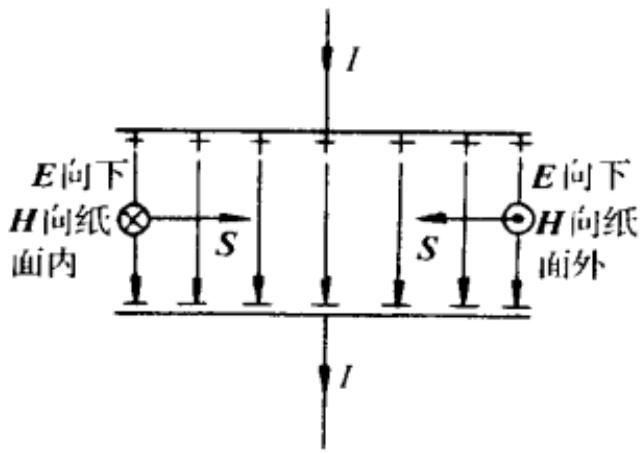
\includegraphics[width=0.5\linewidth]{figures/fig_12_2_12_1.jpg}
\end{center}
\begin{center}
    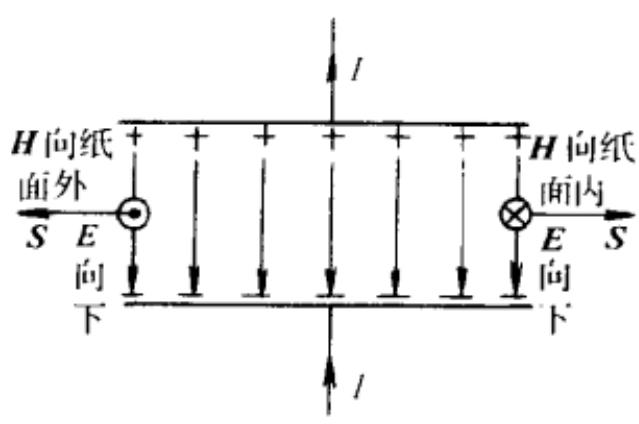
\includegraphics[width=0.5\linewidth]{figures/fig_12_2_12_2.jpg}
\end{center}

\vfill

\textbf{12.2.13.} 一螺线管长为 $l$ ，横截面的半径为 $a (a \ll l)$ ，由 $N$ 匝表面绝缘的细导线密绕而成。略去边缘效应。（1）当导线中的电流为 $I$ 时，试求管内磁场的能量 $W_{m}$ ；（2）当 $I$ 增大时，试说明能量是怎样进入管内的；（3）当电流从零增大到 $I$ 时，试证明进入管内的能量等于管内的磁场能量。

\vfill

\newpage

\textbf{12.2.14.} 半径为 $a$ 的长直导线载有电流 $I, I$ 沿轴线方向并均匀分布在横截面上. 试证明: (1) 在导线表面上, 坡印亭矢量 $\mathbf{S}$ 的方向处处垂直于表面并向内; (2) 导线体内消耗的焦耳热等于 $\mathbf{S}$ 输送来的能量.

\vfill

\textbf{12.2.15.} 一同轴电缆由两个共轴的长直导体圆筒构成, 它们的半径分别为 $a$ 和 $b$ , 如图 12.2.15 所示. 当这电缆的一端接上负载 $R$ , 另一端加上电压 $U$ 时, 电流在两筒上都是均匀分布的. (1) 试求电缆内的电场强度 $\pmb{E}$ 和磁场强度 $\pmb{H}$ 以及坡印亭矢量 $\pmb{S}$ ; (2) 试论证, 不论电源的正极是接在内筒上还是接在外筒上, $\pmb{S}$ 的方向总是由电源端指向负载端; (3) 试证明, 穿过两筒间横截面的功率等于 $U^2 / R$ , 并说明所得结果的物理意义.

图12.2.15
\begin{center}
    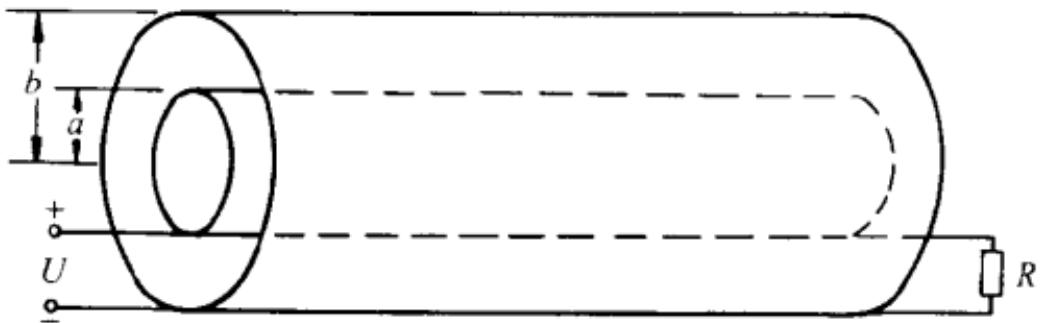
\includegraphics[width=0.5\linewidth]{figures/fig_12_2_15.jpg}
\end{center}

\vfill

\newpage

\textbf{12.2.16.} 氢原子由一个质子和一个电子组成,质子的电荷量为 $e = 1.60 \times 10^{-19}C$ , 电子的电荷量为 -e. 按照经典模型, 电子环绕质子作圆周运动. (1) 试证明: 当电子轨道的半径为 r 时, 氢原子的能量为 $W = -\frac{1}{8\pi\varepsilon_{0}} \frac{e^{2}}{r}$ ; (2) 根据电动力学, 带电粒子作加速运动时, 会向外发出辐射, 对于经典模型的氢原子来说, 由计算得出的辐射功率为①

$$
P = \frac {e ^ {6}}{9 6 \pi^ {3} \varepsilon_ {0} ^ {3} c ^ {3} m ^ {2} r ^ {4}}
$$

式中 $c = 3.00 \times 10^{8} ~m/s$ 是真空中光速, $m = 9.11 \times 10^{-3} ~l ~kg$ 是电子质量. 试由以上两式求 r 与 t 的关系; (3) 设开始时, 氢原子处在基态, 即电子在半径为 $r_{0} = 5.29 \times 10^{-11} ~m$ 的圆轨道上环绕质子运动. 试问它经过多长时间, 便会落到质子上去?

\vfill

\textbf{12.2.17.} 已知 $\varepsilon_{0}=8.854\times10^{-12}F/m,\mu_{0}=4\pi\times10^{-7}H/m$ ，试求 $\frac{1}{\sqrt{\varepsilon_{0}\mu_{0}}}$ 的单位和数值.

\vfill

\newpage
